\section{Exploratory analyses added after the pre-specified study}\label{sec:explore}

The analyses in this section are in neither the analysis plan nor its amendments. They were run after the study of Sections~\ref{sec:design} and~\ref{sec:results} was complete and the manuscript had first been submitted, to answer questions raised by a referee-style review: whether a more accurate, current forecaster changes the picture, whether the disagreement between accuracy and value rests on one biased forecaster, whether it depends on the scheduling program, and whether the perfect-information benchmark is too myopic. All use the same buildings, tariff T1, base battery and simulation code as the main study, and their code and outputs are in the study repository. As checks, the new code reproduces the no-battery, perfect-information and F5 bills of the main run exactly (largest absolute difference in any monthly bill: \$\res{rvCheckMaxDiff}), refitting F5 reproduces its forecasts exactly, the H1 statistic recomputed by the new code is $\res{rvCheckHone}$, and none of the additional linear programs failed. The results are exploratory and change no reported number.

\begin{table}[t]
\centering
\footnotesize
\caption{Forecasters added after the pre-specified study (exploratory): accuracy and value under the demand-charge tariff with the base battery. Q50--Q95 are LightGBM models with the features and settings of F4 trained on the pinball loss of the stated quantile level (Q90 reproduces F5); B50 and B90 are the median and the 0.9 quantile of the zero-shot foundation model Chronos-Bolt from the same model run; F4 is shown for reference. MAE: median over building-months; share: median over buildings of the annual share of the perfect-information saving; bill up: buildings whose annual bill exceeded the no-battery bill; saving: median over buildings, in per cent of the annual bill and in dollars per kW of battery power per year.}\label{tab:explore}
\setlength{\tabcolsep}{4pt}
\begin{tabular}{lrrrrrr}
\toprule
 & MAE & \multicolumn{2}{c}{Open loop} & \multicolumn{3}{c}{Guarded} \\
\cmidrule(lr){3-4}\cmidrule(lr){5-7}
Forecaster & (kWh/h) & Share & Bill up (\%) & Share & Saving (\%) & \$/kW-yr \\
\midrule
F4 (LightGBM) & \res{rvMaeFfour} & $\res{rvQFfourSh}$ & \res{rvQFfourUp} & \res{rvQGFfourSh} & \res{rvQGFfourPct} & \res{rvQGFfourUsd} \\
Q50 & \res{rvMaeQfifty} & $\res{rvQQfiftySh}$ & \res{rvQQfiftyUp} & \res{rvQGQfiftySh} & \res{rvQGQfiftyPct} & \res{rvQGQfiftyUsd} \\
Q70 & \res{rvMaeQseventy} & $\res{rvQQseventySh}$ & \res{rvQQseventyUp} & \res{rvQGQseventySh} & \res{rvQGQseventyPct} & \res{rvQGQseventyUsd} \\
Q80 & \res{rvMaeQeighty} & $\res{rvQQeightySh}$ & \res{rvQQeightyUp} & \res{rvQGQeightySh} & \res{rvQGQeightyPct} & \res{rvQGQeightyUsd} \\
Q90 (= F5) & \res{rvMaeQninety} & $\res{rvQQninetySh}$ & \res{rvQQninetyUp} & \res{rvQGQninetySh} & \res{rvQGQninetyPct} & \res{rvQGQninetyUsd} \\
Q95 & \res{rvMaeQninetyfive} & $\res{rvQQninetyfiveSh}$ & \res{rvQQninetyfiveUp} & \res{rvQGQninetyfiveSh} & \res{rvQGQninetyfivePct} & \res{rvQGQninetyfiveUsd} \\
\midrule
B50 (Chronos-Bolt) &\res{rvMaeSevenBfifty} & $\res{rvBfiftySh}$ & \res{rvBfiftyUp} & \res{rvGBfiftySh} & \res{rvGBfiftyPct} & \res{rvGBfiftyUsd} \\
B90 (Chronos-Bolt) &\res{rvMaeSevenBninety} & $\res{rvBninetySh}$ & \res{rvBninetyUp} & \res{rvGBninetySh} & \res{rvGBninetyPct} & \res{rvGBninetyUsd} \\
\bottomrule
\end{tabular}
\end{table}

\subsection{A foundation-model forecaster}\label{sec:explore-tsfm}
If accuracy were the problem, a more accurate forecaster should fix it. We added Chronos-Bolt~\cite{ansari2024chronos}, a time-series foundation model, in its small version (\texttt{amazon/chronos-bolt-small}) and zero-shot: at midnight before each day it receives the previous 512 hours of the building's own load, with no temperature and no fitting, and returns quantile forecasts of the next 24 hours. Its median (B50) is the choice that minimises the expected absolute error, and its 0.9 quantile (B90), from the same model run, is the peak-conservative choice that corresponds to F5. Both were scheduled with the program~\eqref{eq:lp} and executed open loop and with the guard.

The median forecast was the most accurate of the seven forecasters: its median monthly MAE was \res{rvMaeSevenBfifty} kWh per hour against \res{rvMaeSevenFfour} for LightGBM with observed temperature (F4), its mean MAE rank among the seven was \res{rvRankSevenBfifty} against \res{rvRankSevenFfour} for F4, and it was more accurate than F4 in \res{rvBfiftyBeatsFfour}\% of building-months. Executed open loop, it was nevertheless as harmful as the other unbiased forecasters: it raised the bill in \res{rvBfiftyUp}\% of buildings, with a median share of $\res{rvBfiftySh}$ (Table~\ref{tab:explore}). Its own 0.9 quantile, less accurate (MAE \res{rvMaeSevenBninety}, mean rank \res{rvRankSevenBninety}) and biased upward by a median \res{rvBiasBninety}\% per month, was the only forecaster run with the plain program whose open-loop schedules saved money in the median building (share \res{rvBninetySh}; a higher bill in \res{rvBninetyUp}\% of buildings), and with the guard it gave the largest median saving of any forecaster in the study, \res{rvGBninetyPct}\% of the bill (\$\res{rvGBninetyUsd} per kW-year), against \res{rvGBfiftyPct}\% (\$\res{rvGBfiftyUsd}) for its own median and \res{pctT1GF4}\% for guarded LightGBM. Across the seven forecasters the mean Kendall $\tau$ between accuracy and value was $\res{rvSevenOpen}$ (CI $\res{rvSevenOpenLo}$ to $\res{rvSevenOpenHi}$) open loop and $\res{rvSevenGuard}$ with the guard, against $\res{rvSevenPin}$ for the 0.9 pinball loss open loop. A more accurate model did not fix the problem; choosing the right quantile of the same model did. The comparison is not like for like and is not meant to rank the two model families: Chronos-Bolt saw no temperature and was not fitted to the buildings, yet was the more accurate, and the point is that its higher accuracy did not bring higher value. Whether the model's pretraining data include any of these buildings was not checked; an overlap would flatter the accuracy of both of its forecasts rather than create the difference between them.

\subsection{Value against the quantile level}\label{sec:explore-quant}
F5 is a single biased forecaster, so the disagreement between MAE and value might rest on it. We therefore trained LightGBM with the features and settings of F4 on the pinball loss of the quantile levels 0.5, 0.7, 0.8, 0.9 and 0.95. Table~\ref{tab:explore} and Figure~\ref{fig:quant} show a dose-response. As the level rose from 0.5 to 0.95, accuracy fell (median monthly MAE from \res{rvMaeQfifty} to \res{rvMaeQninetyfive} kWh per hour; median monthly relative bias from $\res{rvBiasQfifty}$\% to $\res{rvBiasQninetyfive}$\%), while the median open-loop share rose steadily from $\res{rvQQfiftySh}$ to $\res{rvQQninetyfiveSh}$ and the guarded share from \res{rvQGQfiftySh} to \res{rvQGQninetyfiveSh}. Among the five quantile models the less accurate model was the more valuable one: the mean Kendall $\tau$ between accuracy (negative MAE) and share was $\res{rvQonlyOpen}$ (CI $\res{rvQonlyOpenLo}$ to $\res{rvQonlyOpenHi}$) open loop and $\res{rvQonlyGuard}$ with the guard. Over all nine forecasters (F1--F4 and the five quantile models) the MAE gave $\tau=\res{rvNineOpen}$ open loop and $\res{rvNineGuard}$ with the guard, whereas the 0.9 pinball loss gave $\res{rvNinePin}$ and the mean under-forecast error $\res{rvNineUnder}$ open loop. Two limits are visible as well. Even the 0.95 quantile raised the bill in \res{rvQQninetyfiveUp}\% of buildings when executed open loop, so a quantile forecast does not replace the guard; and with the guard the gain from the 0.5 to the 0.95 quantile was small, \$\res{rvQGQninetyfiveUsd} against \$\res{rvQGQfiftyUsd} per kW-year.

\begin{table}[t]
\centering
\footnotesize
\caption{The primary test (H1) with a headroom margin $m$ in the day-ahead program (exploratory), demand-charge tariff, base battery: mean per-building Kendall $\tau$ between accuracy and captured share (95\% CI in brackets), share of buildings whose annual bill exceeded the no-battery bill when executed open loop, and the range over F1--F5 of the median guarded saving. The column without a margin is the pre-specified program (corrected simulation v2).}\label{tab:headroom}
\setlength{\tabcolsep}{7pt}
\begin{tabular}{lrrr}
\toprule
 & None & $m=5\%$ & $m=10\%$ \\
\midrule
$\tau$, MAE, open loop & $\res{honeMean}$ & $\res{rvHfiveOpen}$ & $\res{rvHtenOpen}$ \\
\quad 95\% CI & [$\res{honeLo}$, $\res{honeHi}$] & [$\res{rvHfiveOpenLo}$, $\res{rvHfiveOpenHi}$] & [$\res{rvHtenOpenLo}$, $\res{rvHtenOpenHi}$] \\
$\tau$, MAE, guarded & $\res{honebMean}$ & $\res{rvHfiveGuard}$ & $\res{rvHtenGuard}$ \\
$\tau$, 0.9 pinball loss, open loop & $\res{pinOpenMean}$ & $\res{rvHfivePin}$ & $\res{rvHtenPin}$ \\
$\tau$, MAE, F1--F4, open loop & $\res{fourOpenMean}$ & $\res{rvHfiveFour}$ & $\res{rvHtenFour}$ \\
Bill up, open loop, F1--F4 (\%) & \res{negOpenFourLo}--\res{negOpenFourHi} & \res{rvHfiveUpFourLo}--\res{rvHfiveUpFourHi} & \res{rvHtenUpFourLo}--\res{rvHtenUpFourHi} \\
Bill up, open loop, F5 (\%) & \res{negT1F5} & \res{rvHfiveFfiveUp} & \res{rvHtenFfiveUp} \\
Guarded saving (\% of bill) & \res{pctT1GF4}--\res{pctT1GF5} & \res{rvHfiveGPctLo}--\res{rvHfiveGPctHi} & \res{rvHtenGPctLo}--\res{rvHtenGPctHi} \\
\bottomrule
\end{tabular}
\end{table}

\begin{figure}[t]
\centering
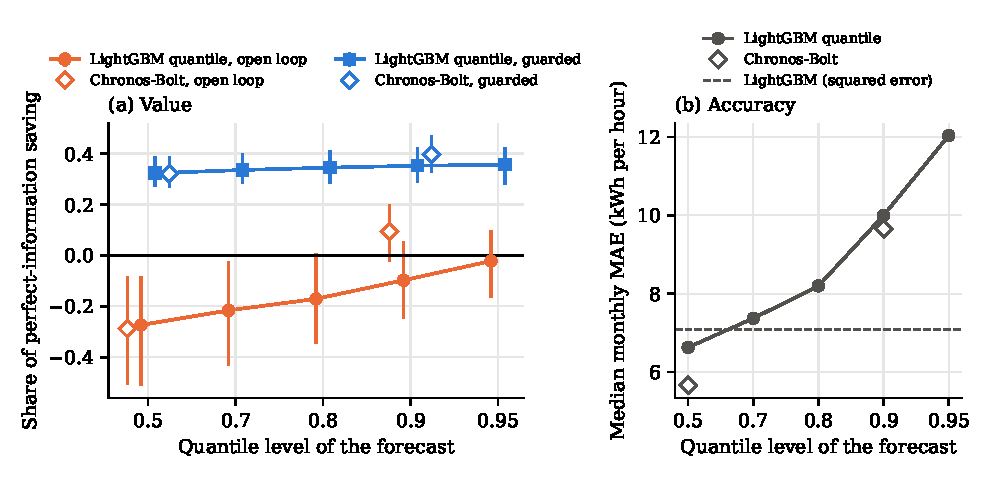
\includegraphics[width=\linewidth]{figures/fig_quantile_value.pdf}
\caption{Value and accuracy against the quantile level of the forecast (exploratory, added after the pre-specified study; demand-charge tariff, base battery). (a) Annual share of the perfect-information saving, medians and interquartile ranges over \res{nKept} buildings, for LightGBM quantile models (filled markers) and for the median and 0.9 quantile of the zero-shot Chronos-Bolt model (open diamonds), open loop and guarded. (b) Median monthly MAE; the dashed line is LightGBM trained on the squared error (F4).}\label{fig:quant}
\end{figure}

\subsection{A headroom margin in the day-ahead program}\label{sec:explore-headroom}
The open-loop failures arise because the program~\eqref{eq:lp} charges until the forecast grid draw touches the month-to-date peak (Section~\ref{sec:results}). The simplest robust remedy is a margin: we added the constraint $g_t+m\hat L_t\le z$, which keeps the planned grid draw at least a fraction $m$ of the forecast load below the planned peak, with $m=5\%$ and $10\%$. The margin changes the answer to H1 (Table~\ref{tab:headroom}). With $m=10\%$ the mean Kendall $\tau$ between MAE and value was $\res{rvHtenOpen}$ (CI $\res{rvHtenOpenLo}$ to $\res{rvHtenOpenHi}$) open loop and $\res{rvHtenGuard}$ with the guard. The null result of H1 is therefore specific to the plain program; with a robust margin, accuracy carries some information about value. The asymmetric score remained more informative ($\tau=\res{rvHtenPin}$ for the 0.9 pinball loss), F5 remained the most valuable of the five forecasters under both controllers, and the margin reduced but did not remove the open-loop damage: the four unbiased forecasters still raised the bill in \res{rvHtenUpFourLo}--\res{rvHtenUpFourHi}\% of buildings, against \res{rvHtenFfiveUp}\% for F5, the only one of the five with a positive median open-loop share ($\res{rvHtenFfiveSh}$). The guard remained the larger lever; combined with the 10\% margin it raised the median guarded saving to \res{rvHtenGPctLo}--\res{rvHtenGPctHi}\% of the bill.

\subsection{Accuracy at a fixed bias}\label{sec:explore-fe}
If accuracy were irrelevant, a lower MAE would not help even among forecasters with the same bias. A within-building regression of the annual share of F1--F5 on their relative MAE and relative bias, with building fixed effects and standard errors clustered by building (\res{rvFeN} building-forecaster observations), separates the two. Open loop, a percentage point of relative MAE changed the share by $\res{rvFeMaeOpen}$ (standard error \res{rvFeMaeSeOpen}) and a percentage point of over-forecast bias by $\res{rvFeBiasOpen}$ (\res{rvFeBiasSeOpen}); with the guard the MAE coefficient was similar, $\res{rvFeMaeGuard}$ (\res{rvFeMaeSeGuard}), and the bias coefficient almost vanished, $\res{rvFeBiasGuard}$ (\res{rvFeBiasSeGuard}). Accuracy therefore matters once the sign of the error is held fixed. The MAE fails as a ranking because the most valuable forecaster is the biased one, and the guard removes most of the reward for bias.

\subsection{A monthly hindsight benchmark}\label{sec:explore-hind}
The perfect-information benchmark is the daily program run on the actual load, which cannot plan the battery across the days of a month. A linear program over each whole calendar month with the actual load, the monthly hindsight optimum, bounds it. Under T1 the hindsight optimum saved a median \res{rvHindPct}\% of the annual bill against \res{rvHindDailyPct}\% for the daily benchmark, so that the daily benchmark captured a median \res{rvHindCapt}\% of the hindsight saving (interquartile range \res{rvHindCaptLo}--\res{rvHindCaptHi}\%); under T2 it captured \res{rvHindCaptTtwo}\%. Measured against the hindsight optimum instead of the daily benchmark, the median annual shares of the five forecasters, open loop and guarded, and of the reactive rule changed by at most \res{rvHindMaxDiff} (guarded F5, for example: \res{rvHindShGF5}). The myopia of the benchmark is therefore small here and does not explain the results.
